\documentclass{beamer}
\usepackage{tikz}
\usepackage{tikz-qtree}
\usepackage{gillius}
\usepackage{mathdots}
\usepackage{abraces}
\usepackage{etex}
\usepackage{nicefrac}

\usetikzlibrary{shapes}
\usetikzlibrary{arrows}
\usetikzlibrary{positioning}
\usetikzlibrary{decorations.pathreplacing}
\usetikzlibrary{decorations.pathmorphing}

\usetheme[everytitleformat=regular]{m}
\setbeamertemplate{navigation symbols}{}

\title{Phylogenetic clustering with a Markov-modulated Poisson process}
\author[RM \& AFYP]{Rosemary McCloskey and Art FY Poon}
\institute[UBC \& BCCfE]{BC Centre for Excellence in HIV/AIDS \\ University of British Columbia}
\date{October 12, 2015}

\graphicspath{{figures/}}

\newcommand{\dd}[2]{\frac{\text{d}\,#1}{\text{d}\,#2}}

\setlength{\parindent}{0pt}

\begin{document}
\definecolor{red}{RGB}{228,26,28}
\definecolor{blue}{RGB}{55,126,184}
\definecolor{green}{RGB}{77,175,74}
\definecolor{purple}{RGB}{152,78,163}

\maketitle
\tableofcontents

\section{Introduction to phylodynamics}

\begin{frame}{Phylogenetic trees}
    \begin{tikzpicture}
        [sibling distance=2.5cm, level distance=2cm]
        \node (root) [circle, draw, very thick, minimum width=0.7cm] { \only<3->{?} };
        \node (fish) [below left=3cm and 1cm of root] {\includegraphics[width=1.8cm]{fish}};
        \node (cat) [below=3cm of root] {\includegraphics[width=1.8cm]{cat}};
        \node (dog) [below right=3cm and 1cm of root] {\includegraphics[width=1.8cm]{dog}};
        \node (cd) [below right=1.5cm and 0.5cm of root, circle, draw, very thick, minimum width=0.7cm] {\only<3->{?}};
        \draw [very thick] (root) -- (fish);
        \draw [very thick] (root) -- (cd) -- (cat);
        \draw [very thick] (cd) -- (dog);

        \uncover<4->{
        \draw [decorate, decoration={brace, amplitude=10pt, mirror}] (dog.north east) -- ++(0cm, 3cm);
        \node [above right=1.5cm and 0.5cm of dog.north east, text width=2.5cm, anchor=west] {evolutionary  relationships};
        }

        \uncover<2->{
        \node (known) [below=1cm of cat] {known species};
        \draw [->, >=stealth] (known) -- (fish);
        \draw [->, >=stealth] (known) -- (cat);
        \draw [->, >=stealth] (known) -- (dog);
        }

        \uncover<3->{
        \node (anc) [above=2cm of fish.west, anchor=south, text width=2cm] {common ancestors};
        \draw [->, >=stealth, shorten >=2mm] (anc) -- (root);
        \draw [->, >=stealth, shorten >=2mm] (anc) -- (cd);
        }

        \uncover<5->{
        \draw [decorate, decoration={brace, amplitude=10pt, raise=5pt}] (root.east) -- (cd.east);
        \node [below right=-0.5 and 1.2cm of root, text width=3cm] {genetic \\ distance \\ or time};
    }
    \end{tikzpicture}
\end{frame}

\begin{frame}{Phylogenetic splits correspond to speciation}
    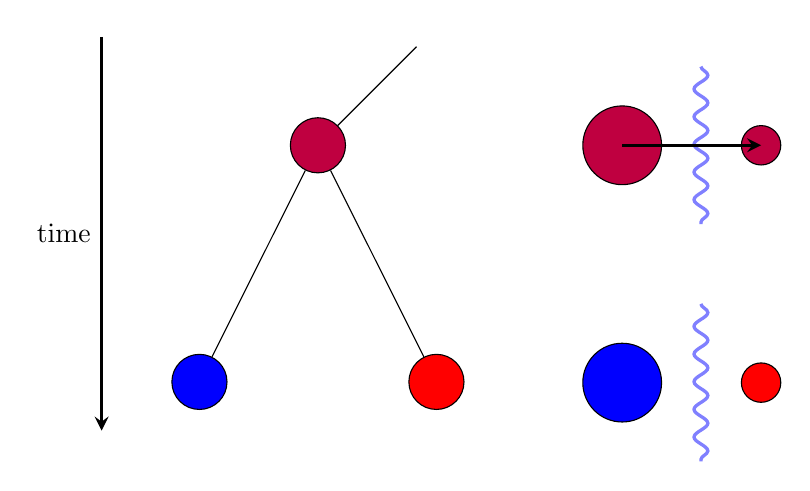
\begin{tikzpicture}
        \node (root) [circle, draw, minimum width=0.7cm, fill=purple] { };
        \node (parent) [above right=of root] { };
        \node (lc) [below left=2.5cm and 1cm of root, circle, draw, fill=blue, minimum width=0.7cm] { };
        \node (rc) [below right=2.5cm and 1cm of root, circle, draw, fill=red, minimum width=0.7cm] { };
        \draw (root) -- (parent);
        \draw (root) -- (lc);
        \draw (root) -- (rc);
        \coordinate [left=4cm of parent] (top);
        \coordinate [below=5cm of top] (bot);
        \draw [->, >=stealth, very thick] (top) -- node [auto, swap] {time} (bot);

        \uncover<2->{
        \node (pop1) [right=3cm of root, circle, fill=purple, minimum width=1cm, draw] { };
        \coordinate [above right=of pop1.center] (rtop);
        \coordinate [below=2cm of rtop] (rbot);
        \draw [decorate, decoration={snake}, blue!50, very thick] (rtop) -- (rbot);
        }

        \uncover<3->{
        \node (pop2) [right=of pop1, circle, fill=purple, minimum width=0.5cm, draw] { };
        \draw (pop1.center) [->, >=stealth, very thick] (pop1.center) -- (pop2.center);
        }

        \uncover<4->{
        \node (pop1a) [below=2cm of pop1, circle, fill=blue, minimum width=1cm, draw] { };
        \node (pop2a) [right=of pop1a, circle, fill=red, minimum width=0.5cm, draw] { };
        \coordinate [above right=of pop1a.center] (rtop);
        \coordinate [below=2cm of rtop] (rbot);
        \draw [decorate, decoration={snake}, blue!50, very thick] (rtop) -- (rbot);
        }
    \end{tikzpicture}
\end{frame}

\begin{frame}{Phylogenetics and viral disease}
    \vspace{-1cm}
    \begin{center}
    \begin{tikzpicture}
        \uncover<1-2>{
        \node (a) {\includegraphics[width=1cm]{hiv}};
        \node at (a.north west) {\includegraphics[width=1cm]{person2}};
        }\uncover<2>{
        \node [right=1.5cm of a] (b) {\includegraphics[width=1cm]{hiv}};
        \node at (b.north west) {\includegraphics[width=1cm]{person1}};
        }
        
        \uncover<3->{
        \node [right=1.5cm of a, opacity=0.4] (b) {\includegraphics[width=1cm]{hiv}};
        \node at (b.north west) [opacity=0.4] {\includegraphics[width=1cm]{person1}};
        \node (a) [opacity=0.4] {\includegraphics[width=1cm]{hiv}};
        \node at (a.north west) [opacity=0.4] {\includegraphics[width=1cm]{person2}};
        }
        
        
        \uncover<2-3>{
        \draw[->, >=stealth, thick] (a) -- (b);
        }\uncover<3->{
        \node [below=2cm of a] (c) {\includegraphics[width=1cm]{hiv}};
        \node at (c.north west) {\includegraphics[width=1cm]{person2}};
        \node [below=2cm of b] (d) {\includegraphics[width=1cm]{hiv}};
        \node at (d.north west) {\includegraphics[width=1cm]{person1}};
        }\uncover<3->{
        \coordinate [left= of a] (timestart);
        \coordinate [left= of c] (timeend);
        \draw[->, >=stealth, thick] (timestart) -- node[auto, swap] {time} (timeend);
        }\uncover<4->{
        \coordinate [right=1.4 of a.center] (root);
        \draw [very thick] (a.center) +(1.4, 0) to +(1.4, 1);
        \draw [very thick] (c.center) -- (root);
        \draw [very thick] (d.center) -- (root);
        \draw [very thick] (root) to +(0, 1);
        }

        \uncover<2->{
        \node (note1) [right= of b, text width=4.5cm] {transmission to new host \\
        $\Rightarrow$ isolated sub-population};
        }
        \uncover<3->{
            \node (note2) [below=0.8cm of note1, text width=4.5 cm] {within-host evolution};
        }
        \uncover<4->{
            \node [below=of note2, text width=4.5 cm] {virus phylogeny \\ $\approx$ transmission tree};
        }

    \end{tikzpicture}

    \uncover<5->{\textbf{phylodynamics}}
    \end{center}
\end{frame}

\section{Motivation: more informed phylogenetic clustering}

\begin{frame}{Phylogenetic clustering}
    \begin{tikzpicture}
        [node distance=0.5, every node/.style={inner sep=-2pt}]
        \node (a) {\includegraphics[width=1cm]{person1}};
        \node [below left=0.5 and 0 of a] (b) {\includegraphics[width=1cm]{person2}};
        \node [right=of a] (c) {\includegraphics[width=1cm]{person3}};
        \node [below=of c] (d) {\includegraphics[width=1cm]{person4}};

        \node (e) [below left=2 and 0.5 of d] {\includegraphics[width=1cm]{person5}};
        \node (f) [right=of e] {\includegraphics[width=1cm]{person6}};

        \node (g) [above right=0.5 and 2 of f] {\includegraphics[width=1cm]{person7}};
        \node (h) [below=of g] {\includegraphics[width=1cm]{person8}};
        \node (i) [above right=0.5 and 0.5 of h] {\includegraphics[width=1cm]{person9}};

        \node (j) [above right=1 and 0.5 of g] {\includegraphics[width=1cm]{person10}};
        \node (k) [right=of j] {\includegraphics[width=1cm]{person11}};
        \node (l) [above right=of k] {\includegraphics[width=1cm]{person12}};

        \draw (a) -- (b) -- (c) -- (a) -- (d) -- (e) -- (f) -- (g) --
        (h) -- (i) -- (g) -- (j) -- (k) -- (l) -- (j) -- (d);
        \draw (b) -- (d);
        
        \uncover<2->{
        \node (groups) [inner sep=5pt, above right=0.5cm and 1cm of a, text width=4.5cm, align=center]
        {groups of epidemiologically \\ related individuals};
        \draw [->, >=stealth, thick] (groups) -- (c);
        \draw [->, >=stealth, thick, shorten >=0.5cm] (groups) -- (k.north);
        }
    \end{tikzpicture}
\end{frame}

\newcommand{\p}[1]{\includegraphics[width=0.7cm, angle=-90]{person#1} 
\includegraphics[width=0.7cm, angle=-90]{hiv}}
\begin{frame}{Clustering by genetic distance}
    \hspace{-0.5cm}
    % http://tex.stackexchange.com/questions/5078/tikz-skipping-levels-when-drawing-trees
    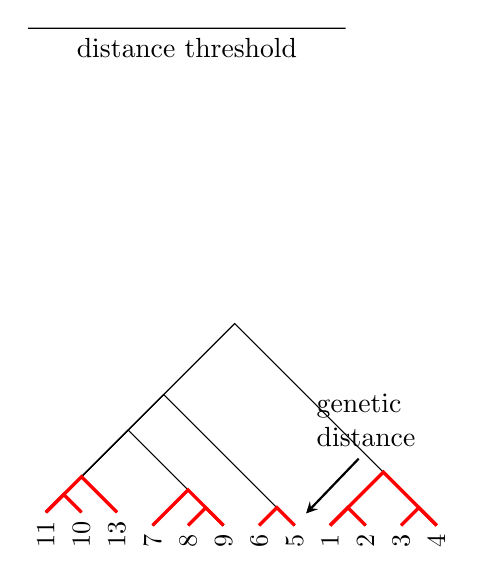
\begin{tikzpicture}[rotate=45, scale=0.95]
    \begin{scope}[rotate=45]
    \node[coordinate] (start) at (0,0) {};
    \xdef\pl{start}
    \foreach \n/\l in {
      \p{11}/p11,
      \p{10}/p10,
      \p{13}/p13,
      \p{7}/p7,
      \p{8}/p8,
      \p{9}/p9,
      \p{6}/p6,
      \p{5}/p5,
      \p{1}/p1,
      \p{2}/p2,
      \p{3}/p3,
      \p{4}/p4%
    } {
      \node[transform shape,below right] (\l) at (\pl.south west) {\n};
      \xdef\pl{\l}
    }
    \end{scope}
    
    \foreach \a/\b in {
      p4/p11,
      p10/p11,
      p13/p11,
      p9/p11,
      p9/p7,
      p9/p8,
      p5/p11,
      p5/p6,
      p2/p1,
      p4/p1,
      p4/p3%
    } {
      \draw (\a.east) |- (\b.east);
    }
    \uncover<2->{
        \draw [red, very thick] (p5.east) |- (p6.east);
        \node (gd) [above right=1cm and 0.5cm of p5, inner sep=0pt, text width=2cm] {genetic \\ distance};
        \draw [->, >=stealth, thick, shorten >=6pt, shorten <=6pt] (gd) -- (p5.east);
    }
    \uncover<3->{
        \draw [red, very thick] (p10.east) |- (p11.east);
        \draw [red, very thick] (p13.east) |- (p11.east);
        \draw [red, very thick] (p9.east) |- (p7.east);
        \draw [red, very thick] (p9.east) |- (p8.east);
        \draw [red, very thick] (p2.east) |- (p1.east);
        \draw [red, very thick] (p4.east) |- (p1.east);
        \draw [red, very thick] (p4.east) |- (p3.east);
        \draw (5, 5) to node [auto, swap] {distance threshold} +(3, -3);
    }
    \end{tikzpicture}
\end{frame}

\begin{frame}{Clustering by genetic distance}
    \begin{tikzpicture}
        [node distance=0.5, every node/.style={inner sep=-2pt}]
        \node (a) {\includegraphics[width=1cm]{person1}};
        \node [below left=0.5 and 0 of a] (b) {\includegraphics[width=1cm]{person2}};
        \node [right=of a] (c) {\includegraphics[width=1cm]{person3}};
        \node [below=of c] (d) {\includegraphics[width=1cm]{person4}};

        \node (e) [below left=2 and 0.5 of d] {\includegraphics[width=1cm]{person5}};
        \node (f) [right=of e] {\includegraphics[width=1cm]{person6}};

        \node (g) [above right=0.5 and 2 of f] {\includegraphics[width=1cm]{person7}};
        \node (h) [below=of g] {\includegraphics[width=1cm]{person8}};
        \node (i) [above right=0.5 and 0.5 of h] {\includegraphics[width=1cm]{person9}};

        \node (j) [above right=1 and 0.5 of g] {\includegraphics[width=1cm]{person10}};
        \node (k) [right=of j] {\includegraphics[width=1cm]{person11}};
        \node (l) [above right=of k] {\includegraphics[width=1cm]{person12}};

        \uncover<1-2> {
        \draw (a) -- (b) -- (c) -- (a) -- (d) -- (e) -- (f) -- (g) --
        (h) -- (i) -- (g) -- (j) -- (k) -- (l) -- (j) -- (d);
        \draw (b) -- (d);
        }
        
        \uncover<2->{
            \draw [red, very thick] (b) -- (a) -- (c);
            \draw [red, very thick] (a) -- (d);
            \draw [red, very thick] (e) -- (f); 
            \draw [red, very thick] (g) -- (i);
            \draw [red, very thick] (j) -- (l);
            \draw [red, very thick] (g) -- (h);
            \draw [red, very thick] (j) -- (k);
        }

        \uncover<4->{
            \draw (a) + (0.4, -0.8) circle (1.8);
            \draw (e) + (0.7, 0) ellipse(1.5 and 0.8);
            \draw [rotate=45] (g) + (-0.1, -0.6) ellipse(1.6 and 1.2);
            \draw [rotate=25] (k) + (0, 0.5) ellipse(2.2 and 1);
        }
    \end{tikzpicture}
\end{frame}

\begin{frame}{Popular problems}
    \begin{columns}
        \begin{column}{0.5\textwidth}
            \includegraphics[width=\textwidth, trim=0 11in 0 0, clip=true]{hughes2009molecular-f1}
        \end{column}
        \begin{column}{0.5\textwidth}
            \includegraphics[width=\textwidth]{lewis2008episodic-f2}
        \end{column}
    \end{columns}
    \begin{columns}
        \begin{column}{0.5\textwidth}
            \tiny
            Hughes, Gareth J., et al. ``Molecular phylodynamics of the heterosexual HIV epidemic in the United Kingdom.'' PLoS Pathog 5.9 (2009): e1000590.
        \end{column}
        \begin{column}{0.5\textwidth}
            \tiny
            Lewis, Fraser, et al. ``Episodic sexual transmission of HIV revealed by molecular phylodynamics.'' PLoS Med 5.3 (2008): e50.
        \end{column}
    \end{columns}
\end{frame}

\begin{frame}{Genetic distance can be misleading}
    \begin{columns}
        \begin{column}{0.5\textwidth}
            \centering
            \includegraphics[height=0.8\textwidth, angle=-90]{fasttree}

            \uncover<2->{
            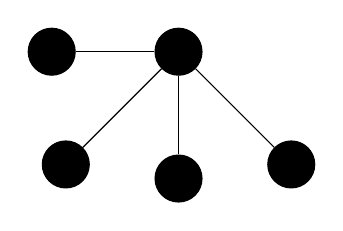
\begin{tikzpicture}
                [every node/.style={circle, draw, fill, inner sep=6pt}]
                \node (a) { };
                \node (b) [below=of a] { };
                \node (c) [below right=of a] { };
                \node (d) [below left=of a] { };
                \node (e) [left=of a] { };
                \draw (a) -- (b);
                \draw (a) -- (c);
                \draw (a) -- (d);
                \draw (a) -- (e);
            \end{tikzpicture}
            }
        \end{column}
        \begin{column}{0.5\textwidth}
            \centering
            \includegraphics[height=0.8\textwidth, angle=-90]{slowtree}

            \uncover<2->{
            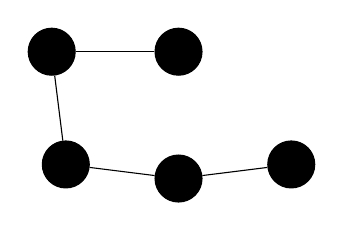
\begin{tikzpicture}
                [every node/.style={circle, draw, fill, inner sep=6pt}]
                \node (a) { };
                \node (b) [below=of a] { };
                \node (c) [below right=of a] { };
                \node (d) [below left=of a] { };
                \node (e) [left=of a] { };
                \draw (a) -- (e);
                \draw (e) -- (d);
                \draw (d) -- (b);
                \draw (b) -- (c);
            \end{tikzpicture}
            }
        \end{column}
    \end{columns}
\end{frame}

\begin{frame}{Clustering by branching rates}
    \only<1>{\includegraphics[height=\textwidth,angle=-90]{pcbr_example}}
    \only<2->{\includegraphics[height=\textwidth,angle=-90]{pcbr_example_color}}

    \hspace{1.2cm}
    \uncover<3->{
    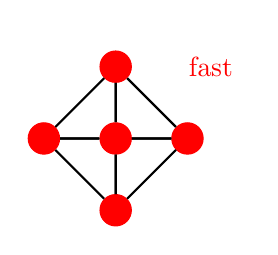
\begin{tikzpicture}
        [node distance=0.5,
         every node/.style={circle, draw=red, fill=red, inner sep=4pt}]
        \node (a) { };
        \node [below=of a] (b) { };
        \node [below=of b] (c) { };
        \node [right=of b] (d) { };
        \node [left=of b] (e) { };
        \draw [thick] (a) -- (b) -- (d) -- (a);
        \draw [thick] (a) -- (b) -- (e) -- (a);
        \draw [thick] (c) -- (b) -- (d) -- (c);
        \draw [thick] (c) -- (b) -- (e) -- (c);
        \node [right=of a, draw=none, fill=none, text=red] {fast};
    \end{tikzpicture}
    }
    \hspace{0.2cm}
    \uncover<4->{
    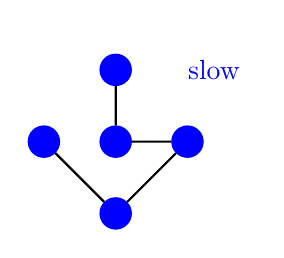
\begin{tikzpicture}
        [node distance=0.5,
         every node/.style={circle, draw=blue, fill=blue, inner sep=4pt}]
        \node (a) { };
        \node [below=of a] (b) { };
        \node [below=of b] (c) { };
        \node [right=of b] (d) { };
        \node [left=of b] (e) { };
        \draw [thick] (a) -- (b) -- (d) -- (c) -- (e);
        \node [right=of a, draw=none, fill=none, text=blue] {slow};
    \end{tikzpicture}
    }
\end{frame}


\section{A Markov-modulated Poisson process on phylogenies}

\begin{frame}{Modelling branching rates}
    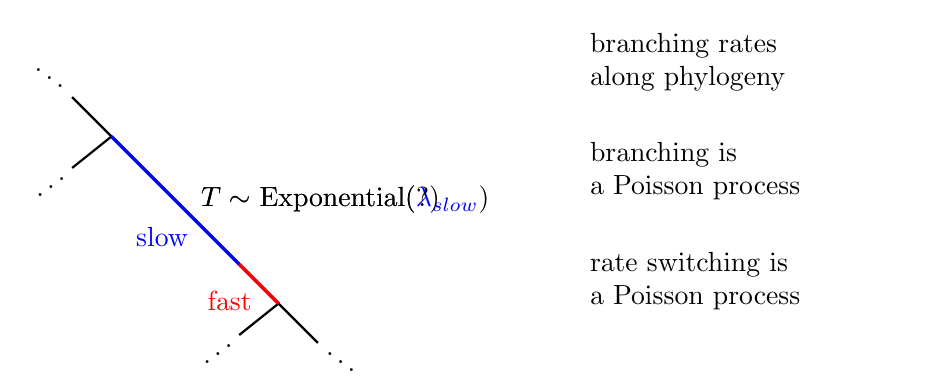
\begin{tikzpicture}
        [every node/.style={inner sep=2pt}]
        \coordinate (a);
        \coordinate [below right=3 of a] (b);
        \draw [thick] (a) -- ++ (-0.5, 0.5) node [anchor=south east] {$\ddots$};
        \draw [thick] (a) -- ++ (-0.5, -0.4) node [inner ysep=-4pt, inner xsep=2pt, anchor=north east] {$\iddots$};
        \draw [thick] (b) -- ++ (-0.5, -0.4) node [inner ysep=-4pt, inner xsep=2pt, anchor=north east] {$\iddots$};
        \draw [thick] (b) -- ++ (0.5, -0.5) node [anchor=north west, inner ysep=-4pt] {$\ddots$};
        \draw [thick] (a) -- (b);
        \uncover<2->{
            \draw [blue, very thick] (a) -- node [auto, swap, text=blue] {slow} (b);
            \node (note1) [above right=0.5 and 6 of a, text width=4cm] {branching rates \\ along phylogeny};
        }
        \uncover<3>{
            \draw [blue] (a) -- node [auto, text=black] {
                $T \sim $ Exponential(\color{blue}$\lambda_\text{slow}$\color{black})
            } (b);
        }
        \uncover<4->{
            \draw [blue] (a) -- node [auto, text=black] {
                $T \sim $ Exponential(?)
            } (b);
        }
        \uncover<3->{
            \node (note2) [below=0.5 of note1, text width=4cm] {branching is \\ a Poisson process};
        }
        \uncover<4->{
            \node [below=0.5 of note2, text width=4cm] {rate switching is \\ a Poisson process};
            \draw [very thick, red] (b) -- node [auto] {fast} ++ (-0.5, 0.5);
        }
    \end{tikzpicture}

    \begin{center}
    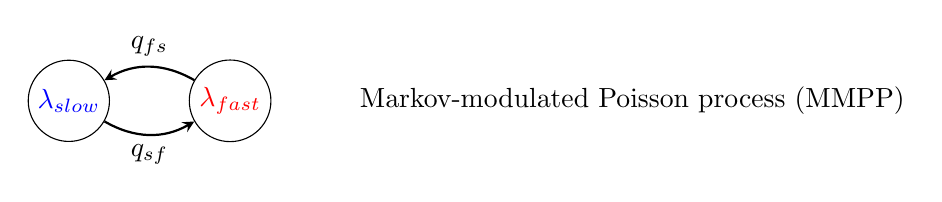
\begin{tikzpicture}
    \uncover<5->{
        \node [circle, draw, text=blue, inner sep=2pt] (slow) {$\lambda_{\text{slow}}$};
        \node [right=of slow, circle, draw, text=red, inner sep=2pt] (fast) {$\lambda_{\text{fast}}$};
        \draw [->, >=stealth, thick] (slow) to [bend right] node[auto, swap] {$q_{sf}$} (fast);
        \draw [->, >=stealth, thick] (fast) to [bend right] node[auto, swap] {$q_{fs}$} (slow);
    }
    \uncover<6->{
        \node [right=of fast] {Markov-modulated Poisson process (MMPP)};
    }
    \end{tikzpicture}
    \end{center}
\end{frame}

\begin{frame}{Markov-modulated Poisson processes}
    \includegraphics[width=\textwidth]{muscariello2004mmpp}

    \includegraphics[width=\textwidth]{ching1997markov}

    \includegraphics[width=\textwidth]{lu2012markov}
\end{frame}

\newcommand{\ls}{\lambda_{\text{slow}}}
\newcommand{\lf}{\lambda_{\text{fast}}}

\begin{frame}[label=steps]{Using the MMPP for clustering}
    \begin{columns}
        \begin{column}{0.5\textwidth}
            \begin{center}
                \textbf{Step 1}
            \end{center}
        \end{column}
        \begin{column}{0.5\textwidth}
            \only<2>{
            \begin{center}
                \textbf{Step 2}
            \end{center}
            }
        \end{column}
    \end{columns}
    \begin{columns}
        \begin{column}{0.5\textwidth}
            \begin{center}
                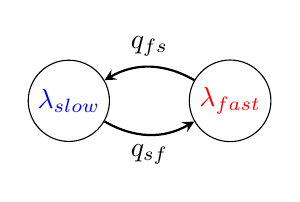
\begin{tikzpicture}
                    \node [circle, draw, text=blue, inner sep=2pt] (slow) {$\lambda_{\text{slow}}$};
                    \node [right=of slow, circle, draw, text=red, inner sep=2pt] (fast) {$\lambda_{\text{fast}}$};
                    \draw [->, >=stealth, thick] (slow) to [bend right] node[auto, swap] {$q_{sf}$} (fast);
                    \draw [->, >=stealth, thick] (fast) to [bend right] node[auto, swap] {$q_{fs}$} (slow);
                \end{tikzpicture}
            \end{center}
        \end{column}
        \begin{column}{0.5\textwidth}
            \only<2->{\includegraphics[height=\textwidth,angle=-90]{pcbr_example_color}}
        \end{column}
    \end{columns}
    \begin{columns}
        \begin{column}{0.5\textwidth}
            Given a phylogeny $T$ with branch lengths, find parameters $\theta$
            to optimize
            \[
                \mathcal{L}(\theta \mid T) = \Pr(T \mid \theta).
            \]
        \end{column}
        \begin{column}{0.5\textwidth}
            \only<2->{
            Given $T$ and $\theta$, find an assignment $\nu$ of states to nodes
            to optimize
            \[
                \Pr(T, \nu \mid \theta).
            \]
        }
        \end{column}
    \end{columns}
\end{frame}

\begin{frame}{MMPP likelihood}
    Recall the likelihood of a realization $D$ of an ordinary Poisson
    process with rate $\lambda$.

    \begin{center}
    \begin{tikzpicture}
        \node at (-0.5, 0) {$D = $};

        \draw (0, 0) -- (4.5, 0);
        \draw (1, -0.1) -- (1, 0.1);
        \draw (3, -0.1) -- (3, 0.1);
        \draw (4.5, -0.1) -- (4.5, 0.1);

        \node at (0.5, -0.3) {$t_1$};
        \node at (2, -0.3) {$t_2$};
        \node at (3.75, -0.3) {$t_3$};
    \end{tikzpicture}
    \end{center}
    \[
        \mathcal{L}(\lambda \mid D) = \color{blue}\lambda\color{black} \times 
        \color{red}\exp(-\lambda t_1)\color{black} \times
        \color{green}\lambda \exp(-\lambda t_2) \lambda \exp(-\lambda t_3)\color{black},
    \]
    \pause
    where
    \begin{align*}
        \color{blue}\lambda &= \text{ arrival rate at time } t_1 \\
        \color{red}\exp(-\lambda t_1) &= \text{ probability of no arrivals by time } t_1 \\
        \color{green}\lambda \exp(-\lambda t_2) \lambda \exp(-\lambda t_3) &= \text{ probability of rest of } D.
    \end{align*}
\end{frame}

\begin{frame}{MMPP likelihood}
    \begin{center}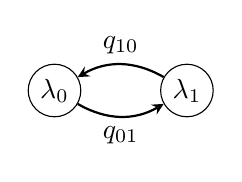
\begin{tikzpicture}
        \node [circle, draw, inner sep=2pt] (slow) {$\lambda_0$};
        \node [right=of slow, circle, draw, inner sep=2pt] (fast) {$\lambda_1$};
        \draw [->, >=stealth, thick] (slow) to [bend right] node[auto, swap] {$q_{01}$} (fast);
        \draw [->, >=stealth, thick] (fast) to [bend right] node[auto, swap] {$q_{10}$} (slow);
    \end{tikzpicture}\end{center}
    \vspace{-1cm}
    Let 
    \begin{itemize}
        \item $\theta = (\lambda_0, \lambda_1, q_{01}, q_{10})$,
            \pause
        \item $P_{ij}(t)$ be the probability that the MMPP is in state $j$
            after time $t$, and that no arrivals have occured by time $t$,
            \pause
        \item $L_i(D) = \mathcal{L}_i(\theta | D)$ be the likelihood of
            $\theta$ given that the Markov chain starts in state $i$.
            \pause
        \item $\pi$ be the equilibrium distribution of the Markov chain.
    \end{itemize}
\end{frame}

\begin{frame}{MMPP likelihood}
    \begin{center}
    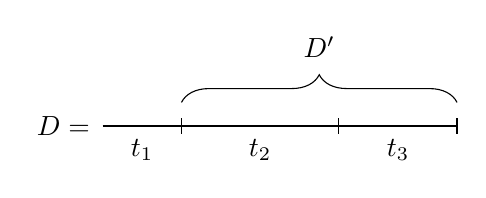
\begin{tikzpicture}
        \node at (-0.5, 0) {$D = $};

        \draw (0, 0) -- (4.5, 0);
        \draw (1, -0.1) -- (1, 0.1);
        \draw (3, -0.1) -- (3, 0.1);
        \draw (4.5, -0.1) -- (4.5, 0.1);

        \draw [decorate, decoration={brace, amplitude=10pt}] (1, 0.3) -- (4.5, 0.3);
        \node at (2.75, 1) {$D'$};

        \node at (0.5, -0.3) {$t_1$};
        \node at (2, -0.3) {$t_2$};
        \node at (3.75, -0.3) {$t_3$};
    \end{tikzpicture}
    \end{center}
    \uncover<2->{
    For the ordinary Poisson process,
    \[
        \mathcal{L}(\lambda \mid D) = \exp(-\lambda t_1) \times \lambda \times 
        \mathcal{L}(\lambda \mid D').
    \]
    }
    \uncover<3->{
    For the MMPP,
    }
    \begin{align*}
        \uncover<3->{L_0(D) &= P_{00}(t_1)\,\lambda_0\,L_0(D')}
        \uncover<4->{ + P_{01}(t_1)\,\lambda_1\,L_1(D')} \\[1em]
        \uncover<5->{
        \mathcal{L}(\theta \mid D) &= \pi_0 L_0(D) + \pi_1 L_1(D)
        }
    \end{align*}
\end{frame}

\begin{frame}{MMPP likeilhood}
    \begin{center}
    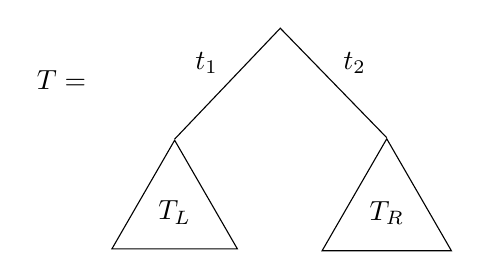
\begin{tikzpicture}
        \coordinate (root);
        \node (lc) [below left=2cm and 1cm of root, regular polygon, regular polygon sides=3, draw] {$T_L$};
        \node (rc) [below right=2cm and 1cm of root, regular polygon, regular polygon sides=3, draw] {$T_R$};
        \draw (lc.north) -- node [auto] {$t_1$} (root) -- node [auto] {$t_2$} (rc.north);
        \node [above left=0.5cm and 1cm of lc.north] {$T = $};
    \end{tikzpicture}
    \end{center}

    For a tree, we take the product of the left and right children's likelihoods.
    \begin{align*}
        L_0(T) = &\left[P_{00}(t_1)\,\lambda_0\,L_0(T_L) + P_{01}(t_1)\,\lambda_1\,L_1(T_L)\right] \\
        \times &\left[P_{00}(t_1)\,\lambda_0\,L_0(T_R) + P_{01}(t_1)\,\lambda_1\,L_1(T_R)\right].
    \end{align*}
\end{frame}

\begin{frame}{Calculating $P_{ij}(t)$}
    Recall $P_{ij}(t)$ is the probability that, after time $t$, no branchings
    have occured \emph{and} the Markov chain is in state $j$, given that the
    Markov chain started in state $i$.
    \begin{align*}
    \uncover<2->{
        P_{ij}(0) &= 
        \begin{cases}
            1 & i = j \\
            0 & \text{otherwise}
        \end{cases} \\
    }\uncover<3->{
        \dd{P_{ij}}{t} &= 
        \begin{cases}
            \sum_{k} P_{ik}(t) q_{kj} & i \neq j \\
            \uncover<4->{P_{ij}(t) (-\sum_{k} q_{jk}) - \lambda_j & i = j.}
        \end{cases}
    }
    \end{align*}

    \tiny
    Fischer, Wolfgang, and Kathleen Meier-Hellstern. ``The Markov-modulated
    Poisson process (MMPP) cookbook.'' Performance evaluation 18.2 (1993):
    149-171.\par
\end{frame}

\begin{frame}{Finally: the likelihood}
    To calculate $\mathcal{L}(\theta \mid T)$:
    \begin{itemize}
        \uncover<2->{
        \item calculate $P_{ij}(t)$ for all states $i, j$ and all branch
            lengths $t$ by numerical integration
        }
        \uncover<3->{
        \item calculate $L_i(T')$ for all states $i$ and all subtrees $T'$ by
            Felsenstein's pruning algorithm (dynamic programming)
        }
    \end{itemize}

    \uncover<4->{
    Optimize $\mathcal{L}(\theta \mid T)$ for $\theta$ using the covariance
    matrix adaptation evolutionary strategy (CMA-ES).
    }

    \tiny
    \vfill
    Hansen, Nikolaus, Sibylle D. Müller, and Petros Koumoutsakos. ``Reducing
    the time complexity of the derandomized evolution strategy with covariance
    matrix adaptation (CMA-ES).'' Evolutionary Computation 11.1 (2003): 1-18.\par
\end{frame}

\againframe<2>{steps}

\begin{frame}{Assigning states to nodes}
    \begin{center}
    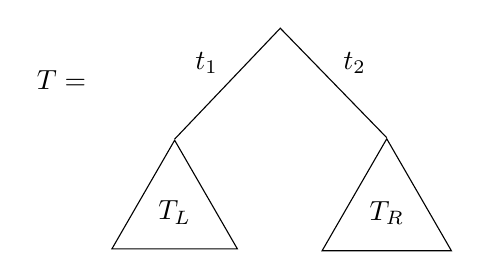
\begin{tikzpicture}
        \coordinate (root);
        \node (lc) [below left=2cm and 1cm of root, regular polygon, regular polygon sides=3, draw] {$T_L$};
        \node (rc) [below right=2cm and 1cm of root, regular polygon, regular polygon sides=3, draw] {$T_R$};
        \draw (lc.north) -- node [auto] {$t_1$} (root) -- node [auto] {$t_2$} (rc.north);
        \node [above left=0.5cm and 1cm of lc.north] {$T = $};
    \end{tikzpicture}
    \end{center}

    \begin{align*}
        L_0(T) = &\uncover<2->{\alert{\max}}\left(P_{00}(t_1)\,\lambda_0\,L_0(T_L) 
        \uncover<2->{,}\uncover<1>{\alert{+}}
        P_{01}(t_1)\,\lambda_1\,L_1(T_L)\right) \times \\
        &\uncover<2->{\alert{\max}}\left(P_{00}(t_1)\,\lambda_0\,L_0(T_R)
        \uncover<2->{,}\uncover<1>{\alert{+}} P_{01}(t_1)\,\lambda_1\,L_1(T_R)\right).
    \end{align*}
\end{frame}

\section{Application: HIV in British Columbia}

\begin{frame}{Human immunodeficiency virus (HIV)}
    \vspace{-0.5cm}
    \begin{center}
    \includegraphics[width=0.75\textwidth]{hiv-structure}
    \end{center}
    \tiny
    By Thomas Splettstoesser (www.scistyle.com) (Own work) [CC BY-SA 4.0
    (http://creativecommons.org/licenses/by-sa/4.0)], via Wikimedia Commons \par
\end{frame}

\begin{frame}{HIV genome}
    \vspace{1cm}

    \includegraphics[width=\textwidth]{hiv-genome}

    \vspace{2cm}
    \tiny
    By Thomas Splettstoesser (www.scistyle.com) (Own work) [CC BY-SA 3.0
    (http://creativecommons.org/licenses/by-sa/3.0) or GFDL
    (http://www.gnu.org/copyleft/fdl.html)], via Wikimedia Commons\par
\end{frame}

\begin{frame}{Making an HIV phylogeny}
    \begin{tikzpicture}

    \end{tikzpicture}
\end{frame}

\begin{frame}{HIV subtype B in British Columbia}
    \tikz[remember picture,overlay] \node [anchor=north east, inner sep=1.8 cm] at (current page.north east) {\includegraphics[width=0.3\textwidth]{timetree-riskgroup-legend}};

    \vspace{-1cm}
    \includegraphics[height=\textwidth,angle=-90]{timetree-riskgroup}
\end{frame}

\begin{frame}{Experimental parameters}
    \begin{description}
        \item[number of rates:] 2, 3, 4
        \item[upper bound on branching rates (branchings/day):] 1, \nicefrac17, \nicefrac{1}{30}
        \item[upper bound on transition rates (transitions/day):] 1, \nicefrac17, \nicefrac{1}{30}
        \item[use tip branches:] yes, no
        \item[branching rates change at nodes only:] yes, no
    \end{description}
\end{frame}

\begin{frame}{3 rates, upper bounds = \nicefrac17}
    \includegraphics[width=\textwidth, trim=0 0 0 0.8in, clip=true]{pcbr1}
\end{frame}

\begin{frame}{4 rates, upper bounds = \nicefrac17, rate changes at nodes}
    \includegraphics[width=\textwidth, trim=0 0 0 0.8in, clip=true]{pcbr2}
\end{frame}

\section{Challenges: validation}

\end{document}

\begin{frame}
    \frametitle{Genetic distance based clustering}
    \tikz[remember picture,overlay] \node [anchor=north east, inner sep=1.5 cm] at (current page.north east) {\includegraphics[width=0.3\textwidth]{timetree-riskgroup-legend}};

    \tikz[remember picture,overlay] \node [anchor=north west, inner ysep=1 cm] at (current page.north west) {\includegraphics[width=0.6\textwidth]{timetree-pd-polar}};

    \tikz[remember picture,overlay] \node [anchor=south east, inner ysep=0 cm] at (current page.south east) {\includegraphics[width=0.6\textwidth]{timetree-riskgroup-polar}};
\end{frame}

\begin{frame}
    \frametitle{Model-based clustering}
    \tikz[remember picture,overlay] \node [anchor=north east, inner sep=1.5 cm] at (current page.north east) {\includegraphics[width=0.3\textwidth]{timetree-riskgroup-legend}};

    \tikz[remember picture,overlay] \node [anchor=north west, inner ysep=1 cm] at (current page.north west) {\includegraphics[width=0.6\textwidth]{timetree_4}};

    \tikz[remember picture,overlay] \node [anchor=south east, inner ysep=0 cm] at (current page.south east) {\includegraphics[width=0.6\textwidth]{timetree-riskgroup-polar}};
\end{frame}

\begin{frame}
    \frametitle{Preliminary comparison}
    \tikz[remember picture,overlay] \node [anchor=north east, inner ysep=1.5 cm, inner xsep=0.5 cm, text width=6cm] at (current page.north east) {$\longleftarrow$ 79 clusters \\ median [IQR] 29 [16-56] individuals};

    \tikz[remember picture,overlay] \node [anchor=north west, inner ysep=1 cm] at (current page.north west) {\includegraphics[width=0.6\textwidth]{cluster4}};

    \tikz[remember picture,overlay] \node [anchor=south west, inner xsep=0.5 cm, inner ysep=1 cm, text width=6cm] at (current page.south west) {\hfill 221 clusters $\longrightarrow$ \\ \hfill median [IQR] 5 [8-15] individuals};

    \tikz[remember picture,overlay] \node [anchor=south east, inner ysep=0 cm] at (current page.south east) {\includegraphics[width=0.6\textwidth]{timetree-pd-polar}};
\end{frame}

\begin{frame}
    \frametitle{Challenges}
    \tikz[remember picture,overlay] \node [anchor=north east, inner ysep=1.5 cm, inner xsep=0.5 cm, text width=6.5cm] at (current page.north east) {$\longleftarrow$ likelihood ratio test doesn't work? \\ $\qquad$ how to define clusters?};

    \tikz[remember picture,overlay] \node [anchor=north west, inner ysep=1 cm] at (current page.north west) {\includegraphics[width=0.6\textwidth]{timetree_6}};

    \tikz[remember picture,overlay] \node [anchor=south west, inner xsep=1.5 cm, inner ysep=1 cm] at (current page.south west) {scaling tip branches $\longrightarrow$};

    \tikz[remember picture,overlay] \node [anchor=south east, inner ysep=0 cm] at (current page.south east) {\includegraphics[width=0.6\textwidth]{timetree-qnorm_3}};
\end{frame}

\begin{frame}
    \frametitle{Acknowledgements}

    \textbf{BC Centre for Excellence in HIV/AIDS} \\
    $\qquad$ Art Poon \\
    $\qquad$ Richard Liang \\
    $\qquad$ Jeffrey Joy \\
    $\qquad$ T. Nguyen \\

    \vspace{3cm}
    \includegraphics[width=0.2\textwidth]{logos/nserc}
    \includegraphics[width=0.35\textwidth]{logos/cfe}
    \includegraphics[width=0.35\textwidth]{logos/btp}
    \includegraphics[width=0.1\textwidth]{logos/ubc}
\end{frame}

\end{document}
